\acresetall

In designing the experiment we knew that frequency noise would be a
primary limiting factor.
For the goal of reaching the quantum noise limit, we can also be limited
by thermal noise of the suspensions and coatings.
Seismic noise can be attenuated quite well by choosing a higher frequency.

With these limitations in mind we designed the trap cavity and the supporting
optics and electronics.

%
% We are targeting an optical spring frequency of about 1kHz because this
% about where we can operate given limited budget for seismic isolation.
% With a 2watt laser and finesse of ~10k we constrain the mass to be no more
% than...
%

% optical spring frequency choice

\section{Design Considerations}
\label{sec:lintrap:design}

We want our optical spring frequency to be high enough so the experiment is
not limited by seismic noise.
Without the resources for elaborate seismic isolation we are limited to single
pendulum isolation stages with a natural frequency of order 1Hz.
At 1kHz we have seismic motion below $10^{-12} \mathrm{m/\sqrt{Hz}}$.
With a pendulum isolation we can attenuate at 1kHz by a factor of $10^{-6}$.
Assuming we have a cavity length of order 30cm we can assume a corresponding
frequency noise of about $1 \mathrm{mHz/\sqrt{Hz}}$.
This is well below the free running laser noise of the NPRO laser of about
$10\mathrm{Hz/\sqrt{Hz}}$ at 1kHz (see section \ref{sec:noise:freq}).

% how to get optical spring frequency

To achieve this resonant frequency we will need to have a small mass.
Just how small is determined by the $\mathrm{dP/dL}$ dependance that gives
us the optical spring constant.
For a high finesse, it can be shown, by taking the derivative of the
intracavity power,
that the maximum spring constant for a given power is approximately
\begin{align}
k &= \frac{3^{5/2} F^2}{\pi \lambda c} P \,.
\end{align}
This gives us a minimum mass of
\begin{align}
m &= 3^{5/2} \frac{F^2}{\pi \lambda c \omega^2_0} P \, .
\end{align}
% which gives a maximum resonant frequency of
% \begin{align}
% f_0 &= \frac{F}{2 \pi} \sqrt{\frac{18 P}{\sqrt{12} \pi \lambda m c }} \\
% &\approx 3.8kHz \,.
% \end{align}
% The frequency in the last step was arrived at by using a finesse of 8200
% with a reasonable input power of 1 Watt.


%
% Need high q suspension for small optic in order for the spring stability to be
% dominated by the optical field.
%

Additionally, we need a high Q suspension for the small optic in order for the
spring stability to be dominated by the optical field.
The optical spring will have fairly low phase since we will be operating a
frequency much lower than the cavity pole.



%
% Frequency noise will dominate experiment.
% We can reduce the effect of frequency noise by using a shorter cavity.
%

We use a smaller cavity in order to reduce the effect of frequency noise.
The frequency noise couples in by the ratio of the cavity length and
laser frequency.


%
% With a negative g-factor we get stable angular modes assuming the other
% mass is heavy.
%

As described in section \ref{sec:II}  if we choose a sufficiently heavy mass for the
input mirror, the angular stability of the small mass is governed by the
following effective angular spring constant,
\begin{align}
T &= \frac{F_0 L}{1 - g_1 g_2} g_1 \theta
\end{align}
By choosing negative g-factors we get the stable angular mode for the small
mirror since the large mirror is essentially fixed.

% This is statically stable, what about dynamic instability due to the cavity
% delay?

%
% Goal for experiment was low noise so that we could turn off active feedback.
%

Ultimately, we wanted to lower the frequency impact of frequency noise, so we
chose a short cavity.
Since the linewidth of the resonance is fixed in terms of cavity length
$ ( \mathrm{FWHM}(m) = \lambda / \mathcal{F} ) $ it is
natural to convert the frequency noise to cavity length.
The cavity length noise is related to the frequency noise by,
\begin{align}
\delta L &= \delta f \frac{L}{f} \, .
\end{align}
By using a shorter cavity, we reduce the effect of frequency noise by geometry
alone.

The cavity length is related to the radius of curvature by the fact that we want
negative g-factors, which constrains the length to 1 to 2 times the radius of
curvature (for the case $g_1 = g_2$).
With the off the shelf substrates available at the time, we chose to use a 5cm
radius of curvature for both input and output mirror.

Incedentally, the sizes of the mirrors available with a 5cm radius of curvature
are quite small.
We chose the smallest one for the output mirror, which gave us a payload mass of
about 0.41 grams, well within our criteria for optical spring resonance frequency.

In order to avoid higher order modes near the resonance we examined the resonance
condition for the first ten orders.
We determined that with a radius of curvature of 5cm, we could avoid these modes
well with a cavity length of 7cm.

These criteria lead us to the experimental parameters listed in table
\ref{tab:lintrap1}.


% Our goal, ultimately, is to demonstrate the angular optical trap described in
% chapter \ref{ch:theory}.
% To get there we need to develop the tools and techniques for generating the
% one-dimensional optical trap.

% The one-dimensional trap has been done before at MIT \cite{Corbitt07}.
% In that experiment they were limited by laser frequency noise.
% Since the frequency noise couples into the experiment by $\frac{L \lambda}{c}$,
% we could improve the frequency noise just by shortening the cavity.

% In choosing a cavity length, we had to balance several factors. We wanted it to
% be short. We had limitations on how close we could get the suspension towers.
% We also wanted to keep a negative $g$ factor, defined by
% \begin{equation}
% g = 1-\frac{L}{R} \;,
% \end{equation}
% in order to avoid Sidles Sigg
% instablity since we are by design operating in a radiation pressure dominated
% regime.
% And finally, we wanted to avoid overlap of higher order modes on the TEM00 mode.

\begin{table}
\begin{center}
\begin{tabular}{|l|l|l|}
  \hline
  \multicolumn{3}{|c|}{Parameters of Trap Cavity} \\
  \hline
  \hline
  Parameter & Value & \\
  \hline
  Cavity Length & 7cm & $L_0$ \\
  Coating Reflectivities & 0.99979 & $r_1,r_2$ \\
  Radius of Curvature & 5cm & $\mathcal{R}_1,\mathcal{R}_2$ \\
  Test Mass Mirror & 0.414g & $m$ \\
  Input Mirror Mass & 300g & $M$ \\
  \hline
\end{tabular}
\end{center}
\caption[Trap Cavity Parameters]{Trap Cavity Parameters for the expermiment.}
\label{tab:lintrap1}
\end{table}


%For the experiment to work, we need to be able to push on the mirror with the
%radiation pressure of the laser.
%For this, we wanted a light mirror suspended in some way to allow it to move.
%Additionally, we need to filter out some background seismic noise in the
%region of the experiment.
%We can do this by suspending each mirror in a pendulum.
%This works well for noise supression at higher frequencies, but hanging a
%pendulum from very thin wires creates a sharp resonance peak in the transfer
%function, meaning that the motion of the mirror will look like a very large
%amplitude sine with a frequency of $\sqrt{g/l}/2\pi$.
%We need a way of damping the motion while giving us the ability to align the
%cavity mirrors.
%Fortunately, the design for such a device exists already for use in LIGO to
%suspend and control some of the smaller optics in the instrument.
%With a bit of modification the LIGO \ac{sos} was exactly what we needed.

%So, we built these structures and borrowed some of the more complicated parts
%from friends.\footnote{It's nice to be in a collaboration}
%Figure \ref{fig:susbig} shows what one of the suspension towers we use looked
%like before the modification described in
%Figure \ref{fig:blades}.

\begin{figure}
\centering
  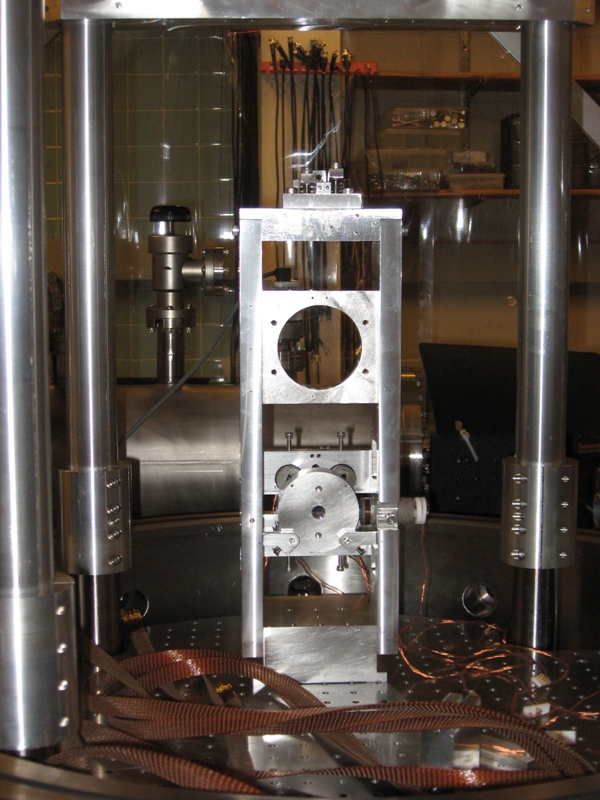
\includegraphics[width=8cm]{./figures/susbig.jpg}
  \caption[Small Optic Suspension]{This shows the full small optic suspension
  tower.
  This is based on the LIGO \ac{sos} design.
  We modified the tower base in order to get the mirrors closer together.
  You can see in this picture the base is flush with the front of the
  vertical side plates.
  This suspension was modified after first cavity lock to further improve
  seismic isolation using blade springs depicted in figure \ref{fig:blades}.
  The extra length of cabling is for suspending the OSEM connection block
  in case the entire platform is suspended as an extra level of seismic
  isolation.
  In this case, suspending the connection block may be desirable to reduce
  seismic coupling to the platform through the stiff vacuum cabling.
  }
  \label{fig:susbig}
\end{figure}

%Another improvement we made was to develop a high-Q glass suspension for the
%small mass. The details of which are described in section \ref{sec:highQsus}.

\begin{figure}
\centering
  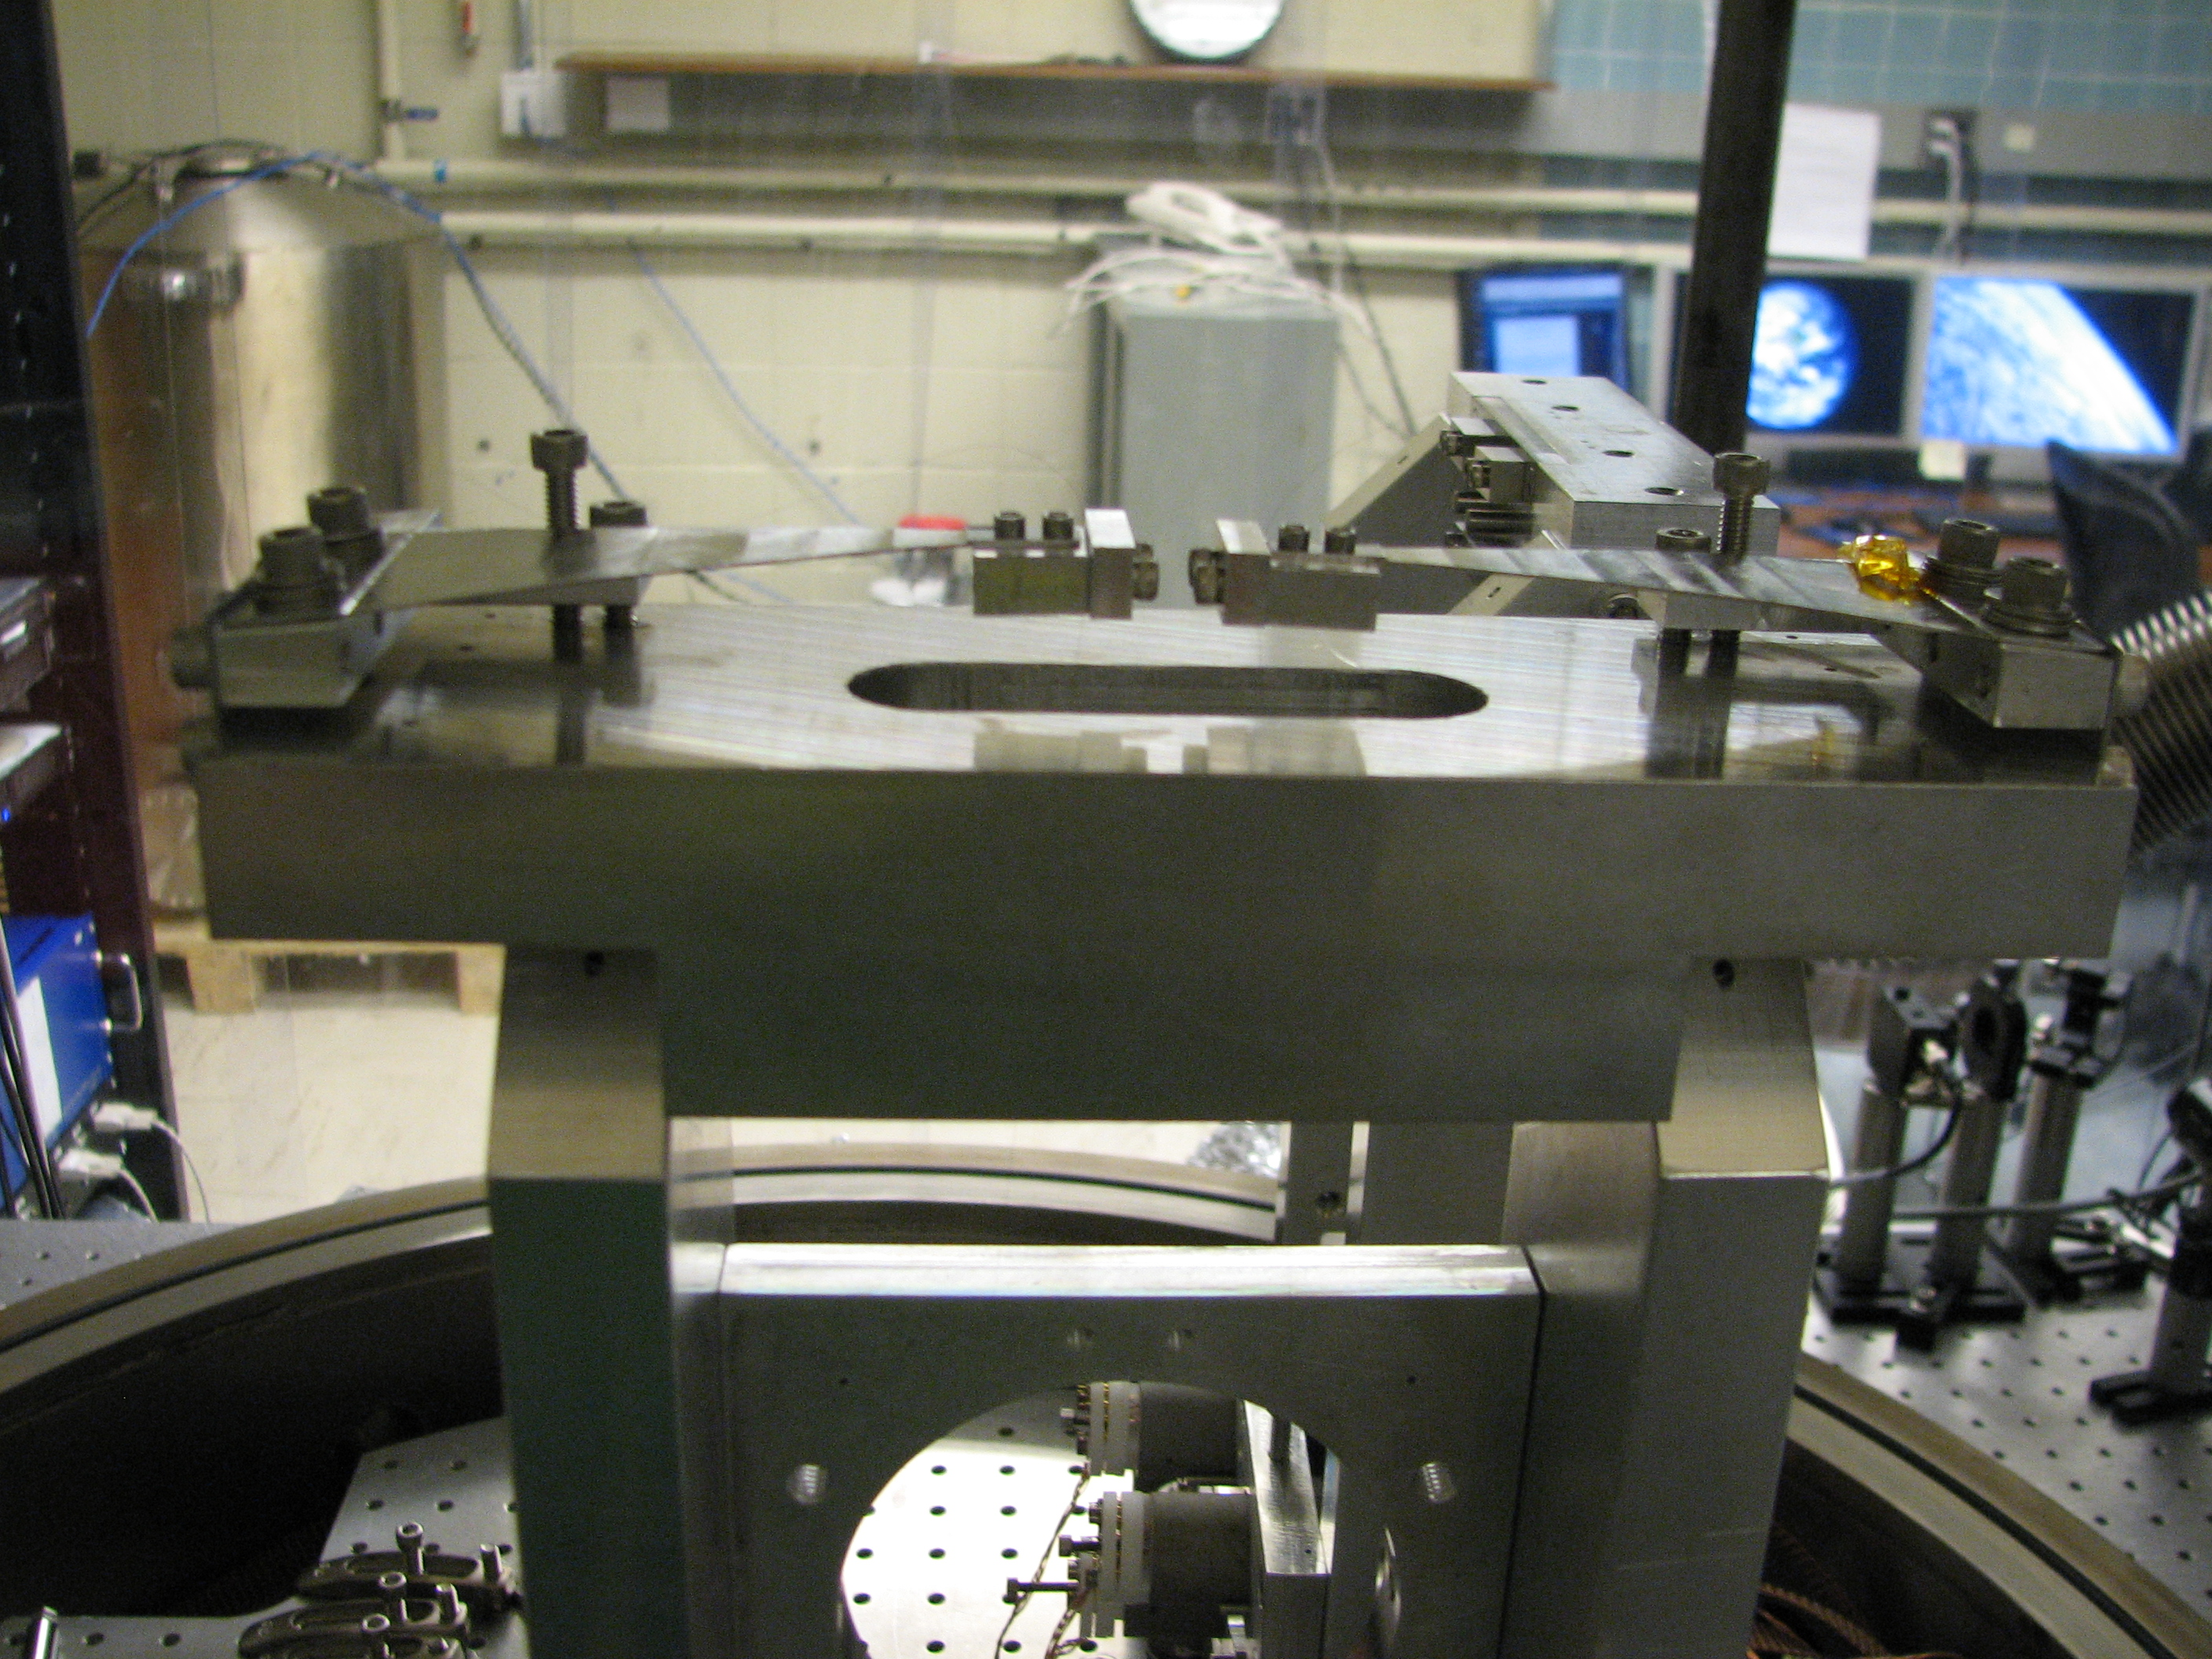
\includegraphics[width=15cm]{./figures/bladesprings.jpg}
  \caption[Blade Spring Modification for Vertical Isolation]{
  This is a picture of the blade springs as installed on one of the suspension
  towers.
  This was necessary for additional bounce mode suppression of seismic noise.
  The bounce mode of the suspension wires were at about 22Hz.
  This unfortunately, was very close to a peak in our seismic spectrum
  resulting in too much vertical motion in our suspended mirrors.
  With the addition of the blade springs, we ended up with a bounce mode of
  about 7Hz providing more supression of the seismic by moving away from a
  seismic peak as well as the additional suppression from a lower frequency
  mode. See section \ref{sec:seismic}.
  }
  \label{fig:blades}
\end{figure}


% \section{Features of Experiment}
% \subsection{High Finesse}
% We need a high finesse cavity to give us the power buildup in the cavity that
% we need for a decent resonant frequency to get beyond some environmental noise.
% Ignoring any damping effects a fairly straight-forward calculation gives the
% resonant frequency we can achieve for a given finesse and input power. For a
% high finesse, it can be shown, by taking the derivative of the intracavity power,
% that the maximum spring constant for a given power is approximately
% \begin{align}
% k &= \frac{18 F^2}{\sqrt{12} \pi \lambda c} P \,,
% \end{align}
% which gives a maximum resonant frequency of
% \begin{align}
% f_0 &= \frac{F}{2 \pi} \sqrt{\frac{18 P}{\sqrt{12} \pi \lambda m c }} \\
% &\approx 3.8kHz \,.
% \end{align}
% The frequency in the last step was arrived at by using a finesse of 8200
% with a reasonable input power of 1 Watt.
% 
% \subsection{Short Cavity}
% \label{sec:lin_short}
% The short cavity gives us a reduction in the frequency noise contribution
% to the noise budget. This reduction scales as the cavity length. This also
% affects the free spectral range, however, and with our finesse, the cavity
% pole is about 140kHz. 

\begin{figure}
\centering
\tikzsetnextfilename{traploops}
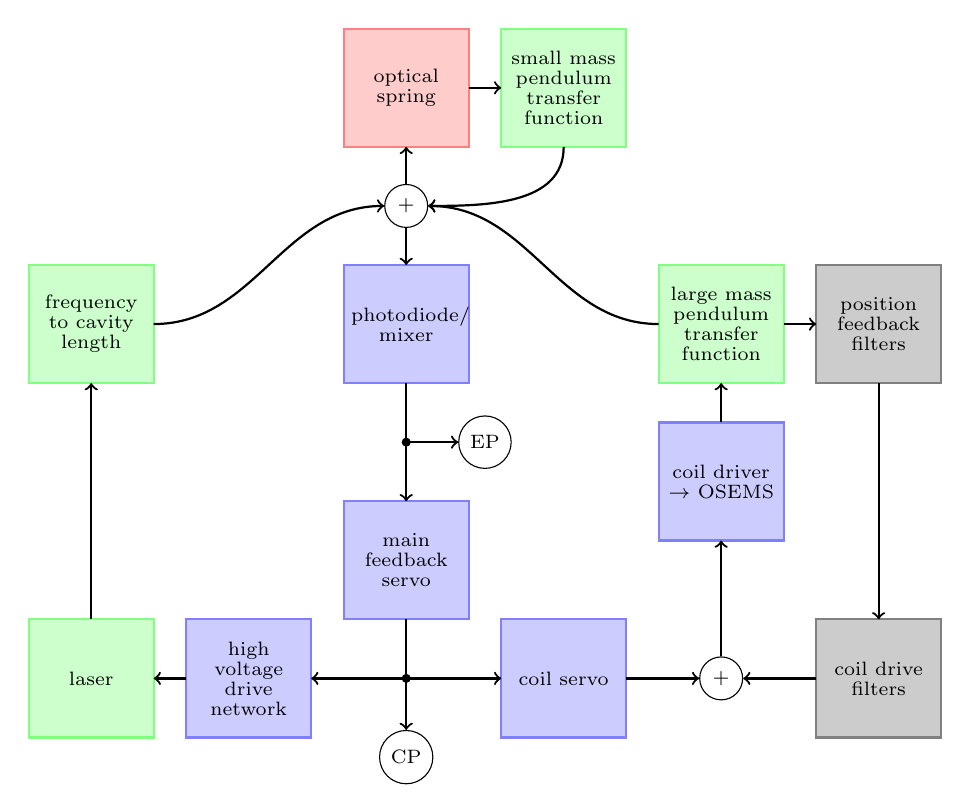
\begin{tikzpicture}
  [analog/.style={rectangle,draw=blue!50,fill=blue!20,thick,align=center,
                  outer sep=0,minimum size=1.5cm,text width=1.4cm},
   digital/.style={rectangle,draw=black!50,fill=black!20,thick,align=center,
                   outer sep=0,minimum size=1.5cm,text width=1.4cm},
   physical/.style={rectangle,draw=green!50,fill=green!20,thick,align=center,
                    outer sep=0,minimum size=1.5cm,text width=1.4cm},
   optical/.style={rectangle,draw=red!50,fill=red!20,thick,align=center,
                   outer sep=0,minimum size=1.5cm,text width=1.4cm},
                   scale=1,
                   every node/.style={scale=1}]
  \renewcommand{\baselinestretch}{0.9}
  \begin{scriptsize}
  \node[circle,draw=black] (sum) at (0,-0.5) {+};
  \node[circle,draw=black] (sumcoil) at (4,-6.5) {+};
  \node[circle,draw,fill=black,minimum size=0.1cm,inner sep=0,outer sep=0] (intersection1) at (0,-3.5) {};
  \node[circle,draw,fill=black,minimum size=0.1cm,inner sep=0,outer sep=0] (intersection2) at (0,-6.5) {};
  \node[analog] (X) at (0,-2) {photodiode/ mixer};
  \node[analog] (F) at (0,-5) {main feedback servo};
  \node[analog] (T) at (2,-6.5) {coil servo};
  \node[analog] (C) at (4,-4) {coil driver $\rightarrow$ OSEMS};
  \node[physical] (P) at (4,-2) {large mass pendulum transfer function};
%  \node[analog] (A) [below=of F] {attenutation for digital system input};
  \node[digital] (D) at (6,-2) {position feedback filters};
  \node[digital] (E) at (6,-6.5) {coil drive filters};
  \node[analog] (H) at (-2,-6.5) {high voltage drive network};
  \node[physical] (L) at (-4,-6.5) {laser};
  \node[physical] (M) at (-4,-2) {frequency to cavity length};
  \node[optical] (O) at (0,1) {optical spring};
  \node[physical] (S) at (2,1) {small mass pendulum transfer function};
  \node[circle,draw=black] (ep) at (1,-3.5) {EP};
  \node[circle,draw=black] (cp) at (0,-7.5) {CP};
  \draw[thick,->] (sum) to (X);
  \draw[thick] (X) to (intersection1);
  \draw[thick,->] (intersection1) to (F);
  \draw[thick] (F) to (intersection2);
  \draw[thick,->] (intersection2) to (T);
  \draw[thick,->] (T) to (sumcoil);
  \draw[thick,->] (sumcoil) to (C);
%  \draw[thick,->] (F) to (A);
  \draw[thick,->] (intersection2) to (H);
  \draw[thick,->] (intersection2) to (cp);
  \draw[thick,->] (H) to (L);
  \draw[thick,->] (L) to (M);
%  \draw[thick,->] (A) to [out=0,in=270] (E);
  \draw[thick,->] (P) to (D);
  \draw[thick,->] (D) to (E);
  \draw[thick,->] (C) to (P);
  \draw[thick,->] (E) to (sumcoil);
  \draw[thick,->] (P) to [out=180,in=0] (sum);
  \draw[thick,->] (sum) to (O);
  \draw[thick,->] (O) to (S);
  \draw[thick,->] (M) to [out=0,in=180] (sum);
  \draw[thick,->] (S) to [out=270,in=0] (sum);
  \draw[thick,->] (intersection1) to (ep);
  \end{scriptsize}
\end{tikzpicture}
\caption[Trapping Loops]{This chart depicts the feedback scheme used for
         locking the trapping cavity and observing the spring behavior.}
\label{fig:traploops}
\end{figure}

\begin{figure}
\centering
\tikzsetnextfilename{scservo}
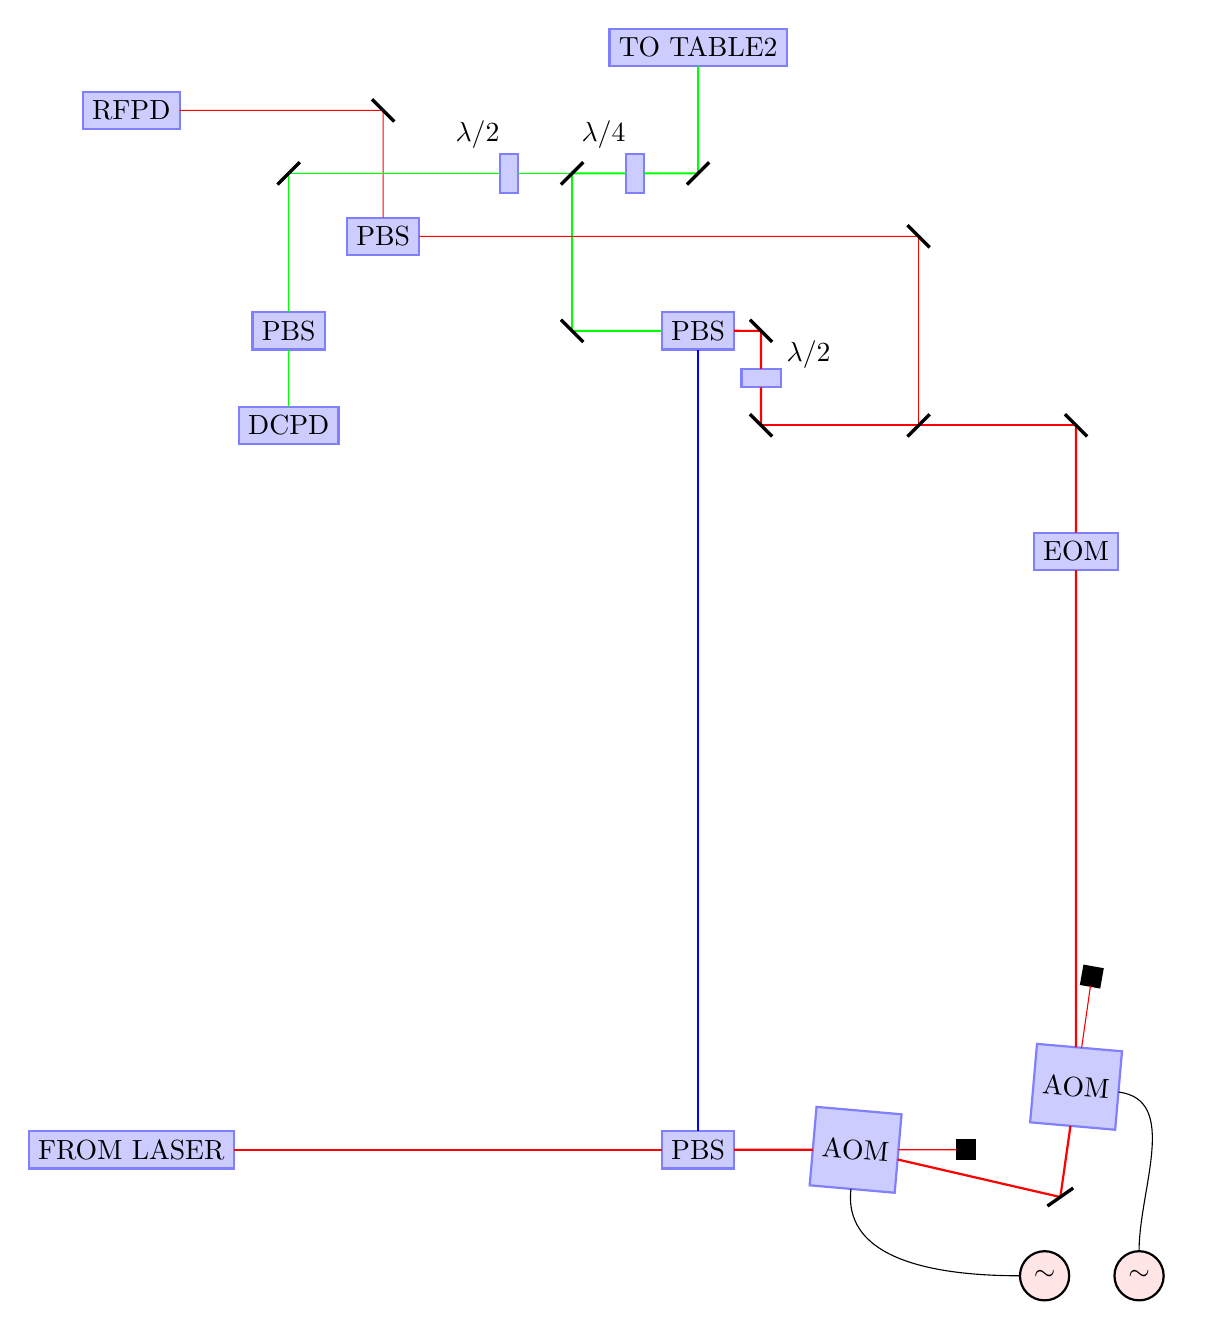
\begin{tikzpicture}
  [scale=0.4,
%  mirror/.style={rectangle,draw=blue!50,fill=blue!20,thick,align=center,
%                  outer sep=0},
  mirror/.style={rectangle,outer sep=0,minimum size=0cm},
  eom/.style={rectangle,draw=blue!50,fill=blue!20,thick,align=center,
                  outer sep=0},
  aom/.style={rectangle,draw=blue!50,fill=blue!20,thick,align=center,
                  outer sep=0,minimum size=1cm},
  pbs/.style={rectangle,draw=blue!50,fill=blue!20,thick,align=center,
                  outer sep=0},
  rfpd/.style={rectangle,draw=blue!50,fill=blue!20,thick,align=center,
                  outer sep=0},
  dcpd/.style={rectangle,draw=blue!50,fill=blue!20,thick,align=center,
                  outer sep=0},
  bblock/.style={rectangle,draw=black,fill=black,thick,align=center,
                  outer sep=0},
  lambdaplate/.style={rectangle,draw=blue!50,fill=blue!20,thick,align=center,
                  outer sep=0},
  beamenter/.style={rectangle,draw=blue!50,fill=blue!20,thick,align=center,
                  outer sep=0},
  beamexit/.style={rectangle,draw=blue!50,fill=blue!20,thick,align=center,
                  outer sep=0},
  osc/.style={circle,draw=black,fill=red!10,thick,align=center,
                  outer sep=0}
                  ]
%  \renewcommand{\baselinestretch}{0.9}

%  \begin{scriptsize}
  \node[beamenter] (laserin) at (-32,7) {FROM LASER};
  \node[beamexit] (laserout) at (-14,42) {TO TABLE2};
  \node[pbs] (pbs1) at (-14,7) {PBS};
  \node[aom,rotate=-5] (aom1) at (-9,7) {AOM};
  \node[bblock] (bb1) at (-5.5,7) {};
  \coordinate (m1) at (-2.5,5.5) {};
  \node[aom,rotate=-5] (aom2) at (-2,9) {AOM};
  \node[bblock,rotate=-10] (bb2) at (-1.5,12.5) {};
  \node[eom] (eom1) at (-2,26) {EOM};
  \coordinate (m2) at (-2,30) {};
  \coordinate (pickoff) at (-7,30) {};
  \coordinate (m4) at (-12,30) {};
  \coordinate (m5) at (-12,33) {};
  \node[pbs] (pbs2) at (-14,33) {PBS};
  \coordinate (m6) at (-18,33) {};
  \coordinate (m7) at (-18,38) {};
  \coordinate (m8) at (-14,38) {};
  \coordinate (m9) at (-7,36) {};
  \node[pbs] (pbs3) at (-24,36) {PBS};
  \coordinate (m10) at (-24,40) {};
  \node[rfpd] (rfpd1) at (-32,40) {RFPD};
  \coordinate (mrefl21) at (-27,38) {};
  \node[pbs] (pbsrefl2) at (-27,33) {PBS};
  \node[dcpd] (dcpd1) at (-27,30) {DCPD};
  \node[lambdaplate,minimum height=0.5cm] (lambda1) at (-16,38) {};
  \node[anchor=south east] (lambdat1) at (-16,38.5) {$\lambda/4$};
  \node[lambdaplate,minimum height=0.5cm] (lambda2) at (-20,38) {};
  \node[anchor=south east] (lambdat2) at (-20,38.5) {$\lambda/2$};
  \node[lambdaplate,minimum width=0.5cm] (lambda3) at (-12,31.5) {};
  \node[anchor=south west] (lambdat3) at (-11.5,31.5) {$\lambda/2$};
  \node[osc] (oscx) at (-3,3) {$\sim$};
  \node[osc] (oscv) at (0,3) {$\sim$};
  \draw[thick,red] (pbs1) to (aom1);
  \draw[thick,red] (aom1) to (m1);
  \draw[red] (aom1) to (bb1);
  \draw[thick,red] (m1) to (aom2);
  \draw[thick,red] (aom2) to (eom1);
  \draw[red] (aom2) to (bb2);
  \draw[thick,red] (eom1) to (m2);
  \draw[thick,red] (m2) to (pickoff);
  \draw[thick,red] (pickoff) to (m4);
  \draw[thick,red] (m4) to (lambda3);
  \draw[thick,red] (lambda3) to (m5);
  \draw[thick,red] (m5) to (pbs2);
  \draw[thick,green] (pbs2) to (m6);
  \draw[thick,green] (m6) to (m7);
  \draw[thick,green] (m7) to (lambda1);
  \draw[thick,green] (lambda1) to (m8);
  \draw[red] (pickoff) to (m9);
  \draw[red] (m9) to (pbs3);
  \draw[red] (pbs3) to (m10);
  \draw[red] (m10) to (rfpd1);
  \draw[thick,blue] (pbs1) to (pbs2);
  \draw[thick,red] (laserin) to (pbs1);
  \draw[thick,green] (m8) to (laserout);
  \draw[green] (m7) to (lambda2);
  \draw[green] (lambda2) to (mrefl21);
  \draw[green] (mrefl21) to (pbsrefl2);
  \draw[green] (pbsrefl2) to (dcpd1);
  \draw[black] (aom1) to [in=180,out=265] (oscx);
  \draw[black] (aom2) to [in=90,out=355] (oscv);
  \draw[black,very thick] (pickoff) ++(225:0.5) -- ++(45:1);
  \draw[black,very thick] (m2) ++(135:0.5) -- ++(315:1);
  \draw[black,very thick] (m1) ++(215:0.5) -- ++(35:1);
  \draw[black,very thick] (m4) ++(135:0.5) -- ++(315:1);
  \draw[black,very thick] (m5) ++(135:0.5) -- ++(315:1);
  \draw[black,very thick] (m6) ++(135:0.5) -- ++(315:1);
  \draw[black,very thick] (m7) ++(225:0.5) -- ++(45:1);
  \draw[black,very thick] (m8) ++(225:0.5) -- ++(45:1);
  \draw[black,very thick] (m9) ++(135:0.5) -- ++(315:1);
  \draw[black,very thick] (m10) ++(135:0.5) -- ++(315:1);
  \draw[black,very thick] (mrefl21) ++(225:0.5) -- ++(45:1);
%  \end{scriptsize}
\end{tikzpicture}
\caption[Subcarrier Servo]{This is a schematic of the optical path for the
         subcarrier servo on Table 1.
         We mix the output of the crystal oscillator with the output of the
         voltage controlled oscillator.
         This is then filtered to give the beat frequency signal which is
         then phase locked to the low frequency function generator.
         }
\label{fig:scservo}
\end{figure}


%\tikzsetnextfilename{gaussian3d}
%\begin{tikzpicture}
%\begin{axis}[
%        view={0}{45},
%        hide axis,
%        xlabel=$x$,ylabel=$y$,
%        mesh/interior colormap name=hot,
%        colormap/blackwhite, 
% ]
%  \addplot3[domain=-1.5:1.5,surf]
%        {exp(-x^2-y^2)};
%\end{axis}
%\end{tikzpicture}

\section{Suspension Systems}

For seismic isolation we have 30cm pendulums attached to the lab optics table.
The table is suspended on pneumatic legs which provide additional isolation
above about 1Hz.
For the input mirror, the mirror is fixed to the pendulum mass.
For the output mirror (payload), the mirror is suspended from the pendulum
mass using thin fibers (see figure \ref{fig:smallsus}).

\begin{figure}
\centering
  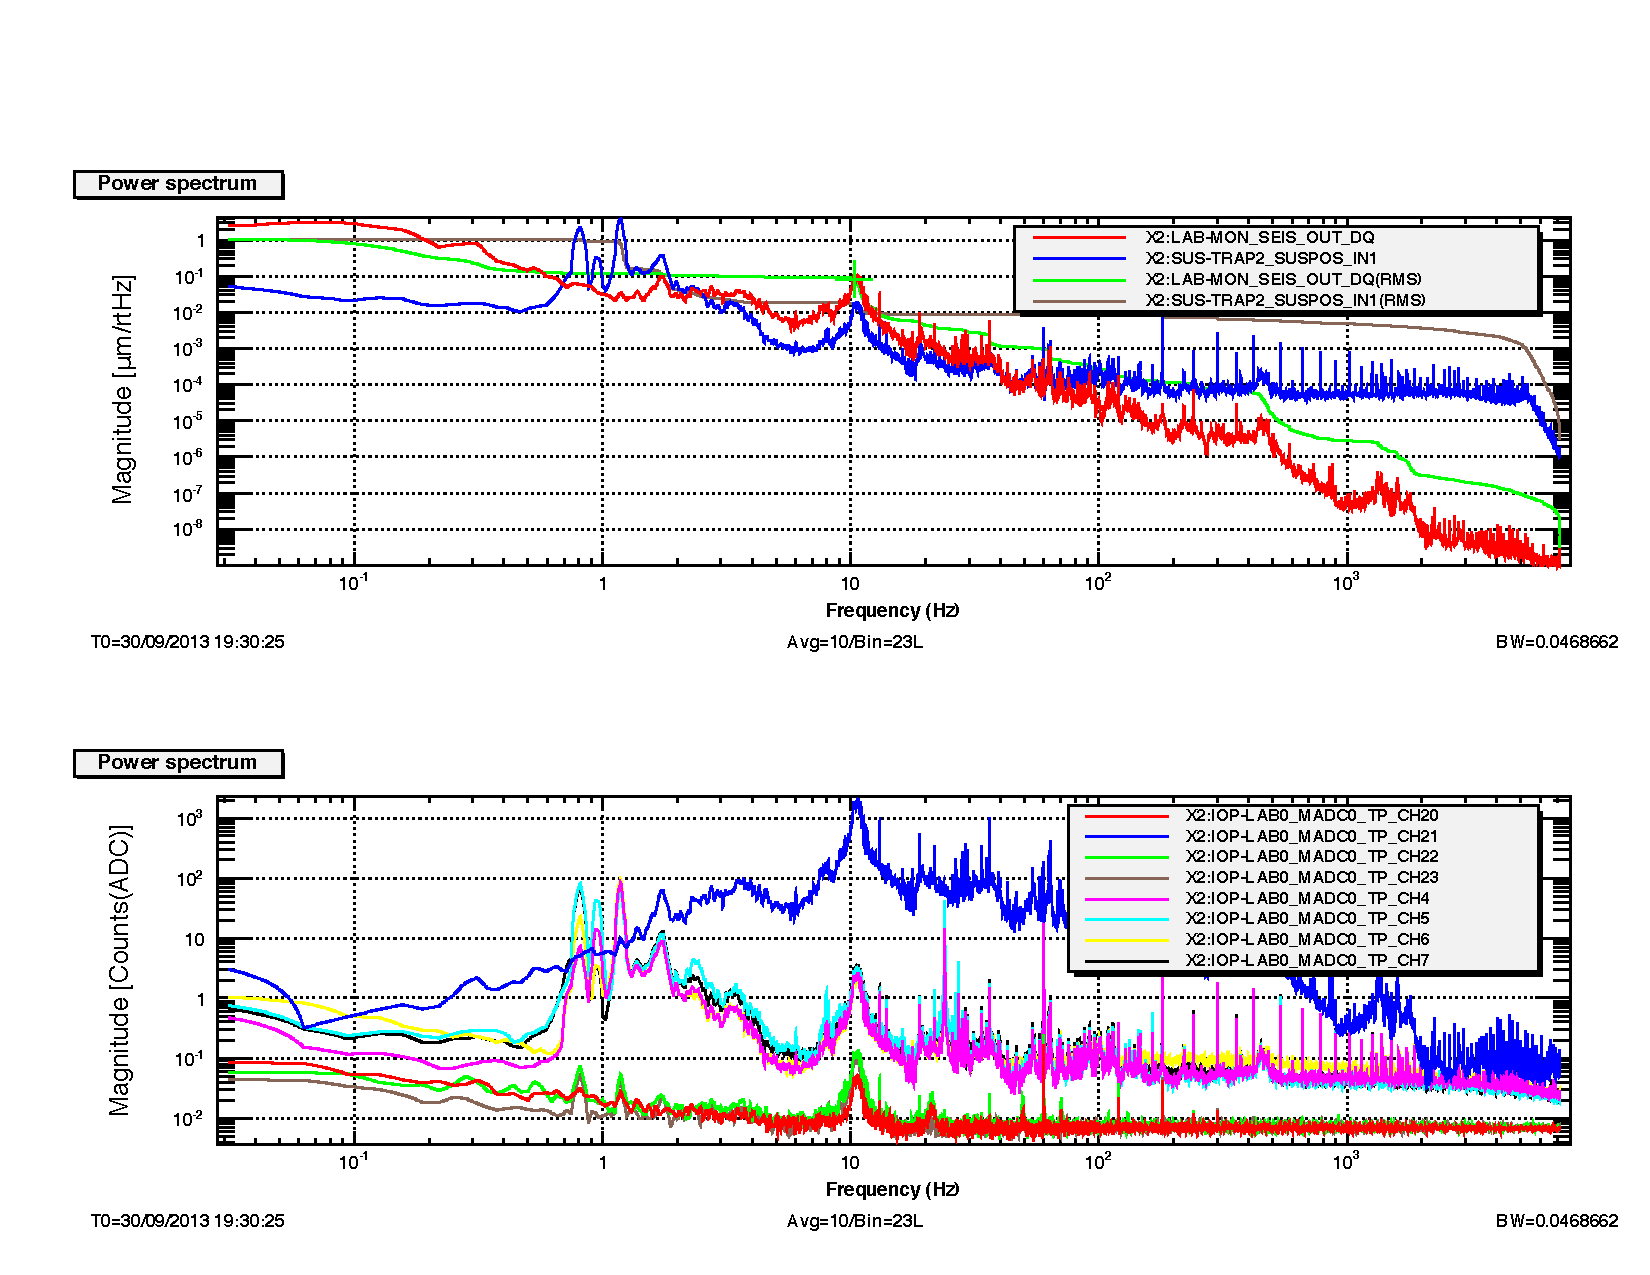
\includegraphics[width=15cm]{./figures/seismic130930.pdf}
  \caption[Background Seismic Noise]{
  background seismic noise.
  The units in the top plot are $\mathrm{\mu m /\sqrt{Hz}}$.
  The bottom plot is in counts from the analog to digital
  converter.
  The red trace in the upper plot is from the seismometer.
  The rms motion due to the noise around 500Hz is about
  $10^{-4}\mu\mathrm{m}/\sqrt{\mathrm{Hz}}$.
  This is about a factor of 10 too much for our experiment
  just from the point of view of the stability criteria.
  The bottom plot of the signals in counts shows the relative
  strength of the signals into the digital system.
  Channels 20, 22, and 23 show the noise floor digital inputs.
  The 10Hz peak shows up in the empty channels due to a small
  amount of crosstalk between channels.
  This plot shows that even though the seismometer input is quite
  high, the amount of crosstalk is low enough to not be a concern
  for us.
  }
  \label{fig:seismicnoise130930}
\end{figure}

\subsection{Payload Suspension}
\label{sec:highQsus}

We want the suspension to have a high Q and low resonant frequency.
The high Q reduces thermal noise in the area of interest
(above the resonant frequency).
And the low resonant frequency gives us better seismic isolation at high
frequencies

With a lower resonant frequency, the response of the mirror due to a force from
radiation pressure is unchanged as long as the resonant frequency is sufficiently lower than the operating frequency. This can be shown by the transfer function of force
applied a mass on a spring. From force to position, this is,
\begin{align}
H &= \frac{1}{k-m\omega^2} \\
  &\approx \frac{1}{-m\omega^2} \; (\omega >> \omega_0)
\end{align}
and is then independant of the spring constant.
The mass acts as a free mass.

For the seismic isolation, however, there is a dependance on the spring constant.
In this case the transfer function from a position displacement at the attachment
point of the spring to the position of the mass looks like,
\begin{align}
H &= \frac{k}{m\omega^2 - k} \\
  &\approx \frac{k}{m\omega^2} \; (\omega >> \omega_0)
\end{align}

In designing the suspension for the small mirror we went through the thermal
noise analysis to determine the best approach. We wanted to suspend the small
mirror using thin glass fibers with a low tension for isolating the mass from
vibrations in the next mass up in the chain.
Thin fused silica fibers are desirable for seismic isolation suspension due to
the very high quality factor acheivable. \cite{Ageev}

The initial thermal noise analysis was for the glue used to mount the glass
fibers to the small mirror. This analysis is described in detail in the
noise chapter. We designed the glue joints of the suspension to minimize
thermal noise based on the analysis. The result of the analysis was to have a
small mass at the glue end of the fiber with a center of gravity close to the
glue surface.

\subsubsection{Glass Fibers}

We needed glass fibers in the final suspension for the high quality factor.
These were produced by heating up a thin section of fused silica and pulling
abruptly while removing the heat.
The resulting fiber has an incredibly high tensile strength and quality factor.

The ratio of tensile strength to weight makes fused silica an ideal material
for seismic isolation.
Seismic isolation is limited by standing waves in the suspension fiber.
This effect is analogous to that from surging in coil springs.
The mass is not as well isolated above the violin modes as the $1/m\omega^2$
of the free mass.
See, for example, Winterflood\cite{0264-9381-19-7-355}.

In our lab we use a small hydrogen and oxygen torch.
The procedure used for the suspension fibers in gravitational wave detectors
is similar except that $\mathrm{CO}_2$ lasers are used instead of a flame
and the process is automated.

Prior to the actual fiber pulling some preparation work with the torch must
be done to get the right shape for the preform.
We prepare the preforms by making a small point on each where the fiber will
connect the two pieces.
The preform work is done with a torch as well.
In our case the preform work was done with a larger torch.
The rod preform is created by heating a rod with a torch and pulling it apart
to form a cone shape at the end of the rod.
The tip of one cone is then used to weld a nub of glass onto the side of the
mirror.
Then, using a small torch we weld the tip of the preforms together and pull
abruptly while removing the torch.

The length and diameter of the fibers can be controlled somewhat and becomes
a bit of an art in practice.
In general, though, one can vary these parameters
through the choice of torch tip size, pressure of gases, and the starting size
and shape of the glass rod.
In the end, generating the right fibers requires the sort of finesse that has
nothing to do with optical cavities.



% We began by gaining experience with welding fibers. In doing so, we decided it
% should not be too difficult to weld the fibers directly to the small mirror.
% This actually proved to be more difficult than anticipated.
% The first attempt at welding a mirror damaged the coating quite visibly even
% though we were careful to shield the coating surface by clamping the mirror
% with quartz tubes.

% After making several improvements to the welding stand, we welded a mirror
% with no visible damage to the coating, however once installed, we found the
% finesse to be too low.
% The mirror was welded, suspended, and placed in vacuum system
% for assembly of the cavity.
% After careful alignment we found the finesse to be about 700, much lower than
% desired.
% Since this was the cavity output mirror that was damaged, it dramatically
% affected the performance of the experiment.
% The power buildup in the cavity is dependent on the
% individual cavity mirror reflectivities.

\subsubsection{Welding Fibers to the Mirror}

The procedure of directly welding to the mirror was a challenge.
The first few attempts produces clearly visible damage.
We needed to protect the coating from the hot gases of the torch
by employing a holder made of graphite.

After upgrading the fiber welding process with the graphite holders we could
weld fibers to the mirror without producing any obvious damage.
The mirror produced from this was used in a cavity with another mirror of the
same coating run.

The finesse of a cavity using mirrors from the same coating run was about 8000
but the finesse of this cavity was only about 800.
The exact nature of this degradation is currently unknown, but since the
finesse is high (800 is still pretty high), the damage to the optic resulted
in only about $0.31\%$ more in additional losses either in absorption or 
scattering.


The order of magnitude lower in finesse was far too much for the
experiment.
So, we came up with a method of glueing the fibers to the mass.

\subsubsection{Glued Fiber Attachements}

It may be that the coating of the welded mirror was damaged directly from the
heat in the substrate,
though the melting point of the Ta2O5 is higher than the temperature of the
substrate during welding. 
It is also quite possible that some of the graphite was deposited onto the
coating and remained despite attempts to clean the coating or that the coating
was damaged during handling.

It would be interesting to find out the exact cause of the damage and possibly
refine the welding procedure.
Though not immediately useful since we decided to go for glueing the fibers to
the small mirror instead.

The final suspension design for this experiment used small cone-shaped glass
nubs at the glue end of the fibers.
This could be constructed monolithicaly
by cold welding\footnote{a process where the substrate is not heated to the
point where the materials flow together} the tip of a glass rod to a small
mirror blank\footnote{or a mirror with a previously damaged coating...} to
create a small nub from which the fiber is pulled.

After creating the glass rod preforms, this procedure is done in one
continuous motion.
The torch is applied to the edge of the mirror blank to
gently heat the point of attachement, then the rod with a sharp point is
placed into the flame to melt the tip and cold weld to the edge of the mirror.
The flame is then directed at the tip of the rod slightly back from the weld
to soften the fiber pull spot.
When the spot is sufficiently heated, the fiber
is pulled away sharply while dropping the flame away from the fiber.
What
remains is a rod attached to a small conical shaped nub monolithically through
a very thin, high Q fiber.

The cold weld allows us to separate this
monolithic fiber assembly because the bond strength is much less than the
yield strength of the fiber.

We then glue this monolithic fiber assembly using the epoxy to the side of the
mirror with undamaged coatings.
This technique allows us to preserve a very high Q ($\approx 5\times 10^5$)
while avoiding damage to the coating.
The results of a Q ringdown measurement can be seen in
figure \ref{fig:Qmeasurement}. 



\begin{figure}
\centering
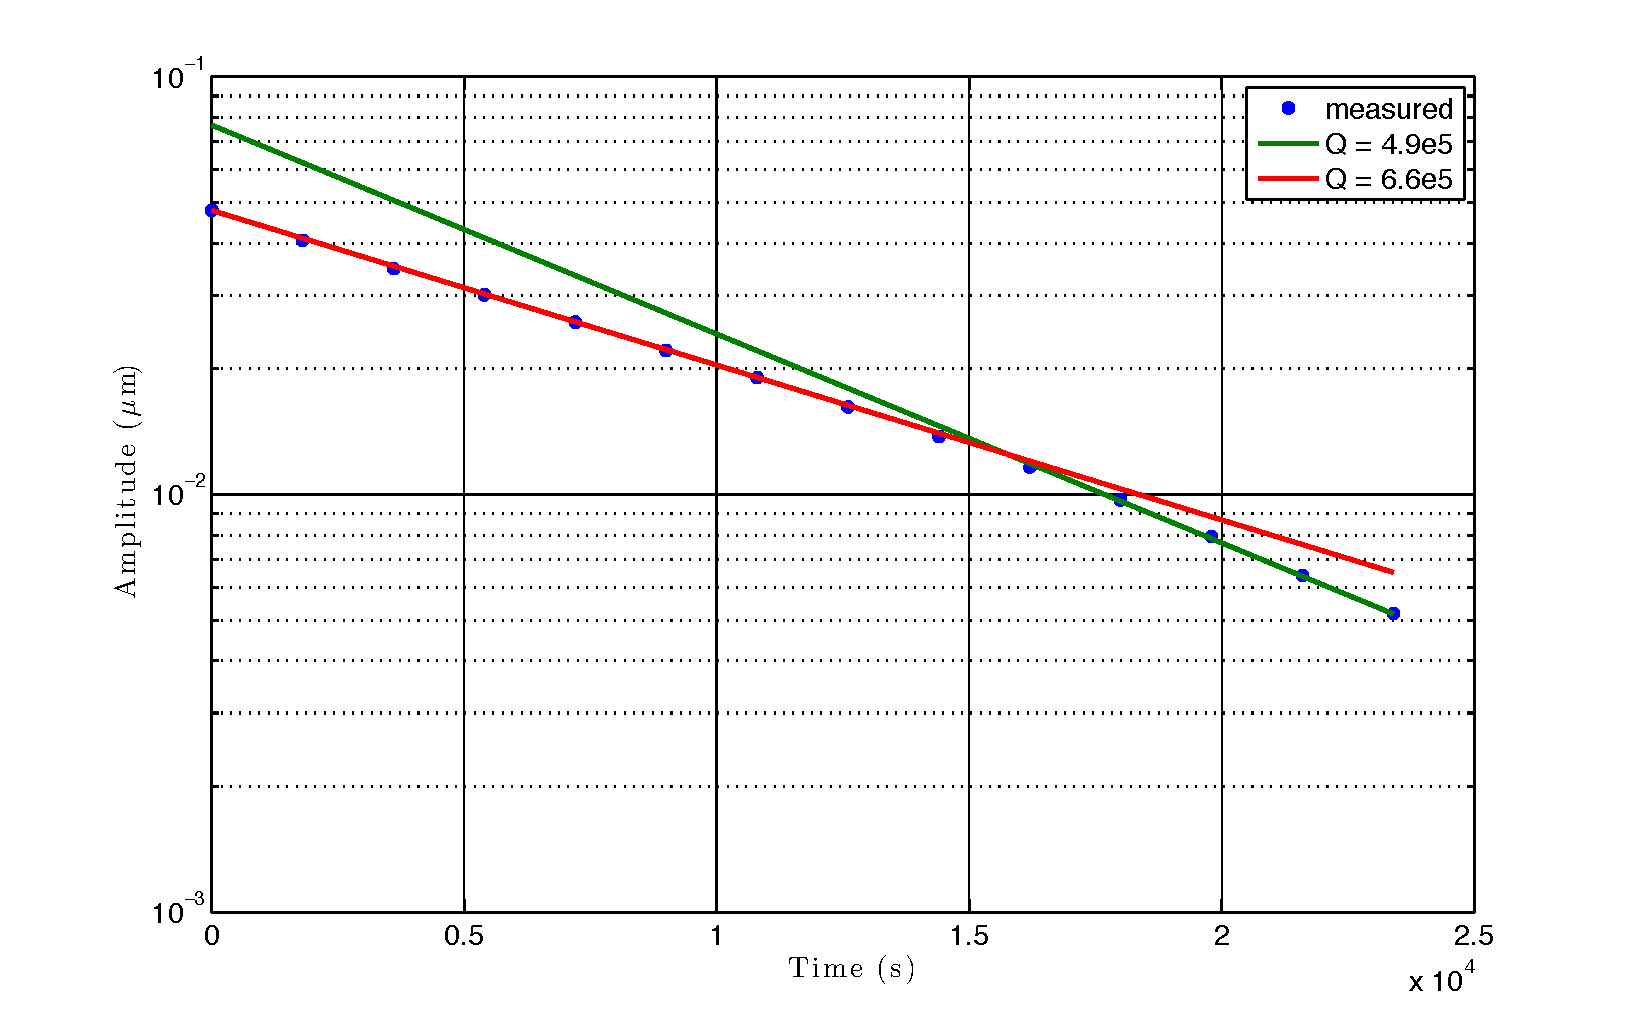
\includegraphics[width=15cm]{./figures/Qmeasurement.pdf}
\caption[Q Measurement of Glass Suspension]{
    This ringdown measurement was done by exciting the $\approx 18\mathrm{Hz}$
    position resonance and measuring the rms motion across the resonant
    frequency from an \ac{asd} measurement of the OSEM position resonance.
    The OSEM position signal is of the metal ring intermediate mass of the
    output mirror suspension as described in section \ref{sec:doublepend}.
    }
\label{fig:Qmeasurement}
\end{figure}

\subsection{Intermediate Suspension}

We have engineered the assembly for the small mirror to have about the
same mass and dimensions as the input mirror assembly.
Both of which fit nicely in a LIGO designed small optic suspension.

The original design of this suspension had no vertical isolation aside
from stretching of the metal suspension wire itself.
This mode was about 22Hz and there was no active damping.
We modified the design to incorporate blade springs for better vertical
isolation with a mode of about 7Hz.
These suspension towers can be seen in figures \ref{fig:susbig} and
\ref{fig:blades}.

The vertical isolation mode is still not damped directly,
although we can damp indirectly since the suspension has some vertical
to horizontal coupling.
We needed to move the resonance frequency away from some large peaks in
the background seismic.
Moving the resonance down in frequency also helps reduce the amount of
vertical seismic motion that couples into the cavity length.

\subsubsection{Double Pendulum}
\label{sec:doublepend}

The output mirror is suspended by glass fibers inside a ring of steel which is
three inches in diameter. The steel ring is the \ac{sos} controlled mass.
Since the mass of the ring is considerably greater than the mass of the small
mirror, the transfer function for force to position on the small mirror can be
approximated by simply the small mirror mass and resonant frequency.
For the complete solution, the equations of motion that need to be solved for
one dimension (per mass) are,
\begin{align}
{F_1}_{\mathrm{ext}} &= m_2a_2-k_2x_2+k_1\left(x_1-x_2\right) \\
{F_2}_{\mathrm{ext}} &= m_1a_1-k_1\left(x_1-x_2\right) \, .
\end{align}
This system can be modelled by a double pendulum as seen in figure
\ref{fig:doublependulum}.
One can also present the equations of motion diagramatically as in figure
\ref{fig:doublesus}.


\begin{figure}
\centering
\tikzsetnextfilename{doublependulum}
\begin{tikzpicture}
  \draw[thick] (-7,0) -- (7,0);
  \draw[gray] (-6.5,0) -- ++(45:1);
  \draw[gray] (-6,0) -- ++(45:1);
  \draw[gray] (-5.5,0) -- ++(45:1);
  \draw[gray] (-5,0) -- ++(45:1);
  \draw[gray] (-4.5,0) -- ++(45:1);
  \draw[gray] (-4,0) -- ++(45:1);
  \draw[gray] (-3.5,0) -- ++(45:1);
  \draw[gray] (-3,0) -- ++(45:1);
  \draw[gray] (-2.5,0) -- ++(45:1);
  \draw[gray] (-2,0) -- ++(45:1);
  \draw[gray] (-1.5,0) -- ++(45:1);
  \draw[gray] (-1,0) -- ++(45:1);
  \draw[gray] (-0.5,0) -- ++(45:1);
  \draw[gray] (0,0) -- ++(45:1);
  \draw[gray] (0.5,0) -- ++(45:1);
  \draw[gray] (1,0) -- ++(45:1);
  \draw[gray] (1.5,0) -- ++(45:1);
  \draw[gray] (2,0) -- ++(45:1);
  \draw[gray] (2.5,0) -- ++(45:1);
  \draw[gray] (3,0) -- ++(45:1);
  \draw[gray] (3.5,0) -- ++(45:1);
  \draw[gray] (4,0) -- ++(45:1);
  \draw[gray] (4.5,0) -- ++(45:1);
  \draw[gray] (5,0) -- ++(45:1);
  \draw[gray] (5.5,0) -- ++(45:1);
  \draw[gray] (6,0) -- ++(45:1);
  \draw[gray] (6.5,0) -- ++(45:1);
  \draw[thick] (0,0) -- (280:10);
  \filldraw[thick,fill=gray!30!white] (280:10.4) circle(0.4);
  \draw[thick] (280:10.4) ++(270:0.4) -- ++(265:1);
  \filldraw[thick,fill=gray!30!white] (280:10.4) ++(270:0.4) ++(265:1) circle(0.2);
  \draw (280:10.4) node(mtwo) {$m_2$};
  \draw (280:10.4) ++(270:0.4) ++(265:1) ++(0.5,0) node(mone) {$m_1$};
\end{tikzpicture}
\caption[Double Pendulum]{The double pendulum system representing the small
    mirror suspension. For small oscillations the pendulum and spring give
    equivalent equations of motion by $k=\sqrt{gm/l}$. $m_1$ represents the
    small mirror and $m_2$ represents the steel ring. If the system depicted
    here was a scale model of the actual small mirror suspension, the relative
    size of the masses and lengths of the pendulums would be more extreme.}
\label{fig:doublependulum}
\end{figure}

\begin{figure}
\centering
\tikzsetnextfilename{doublesus}
\centering
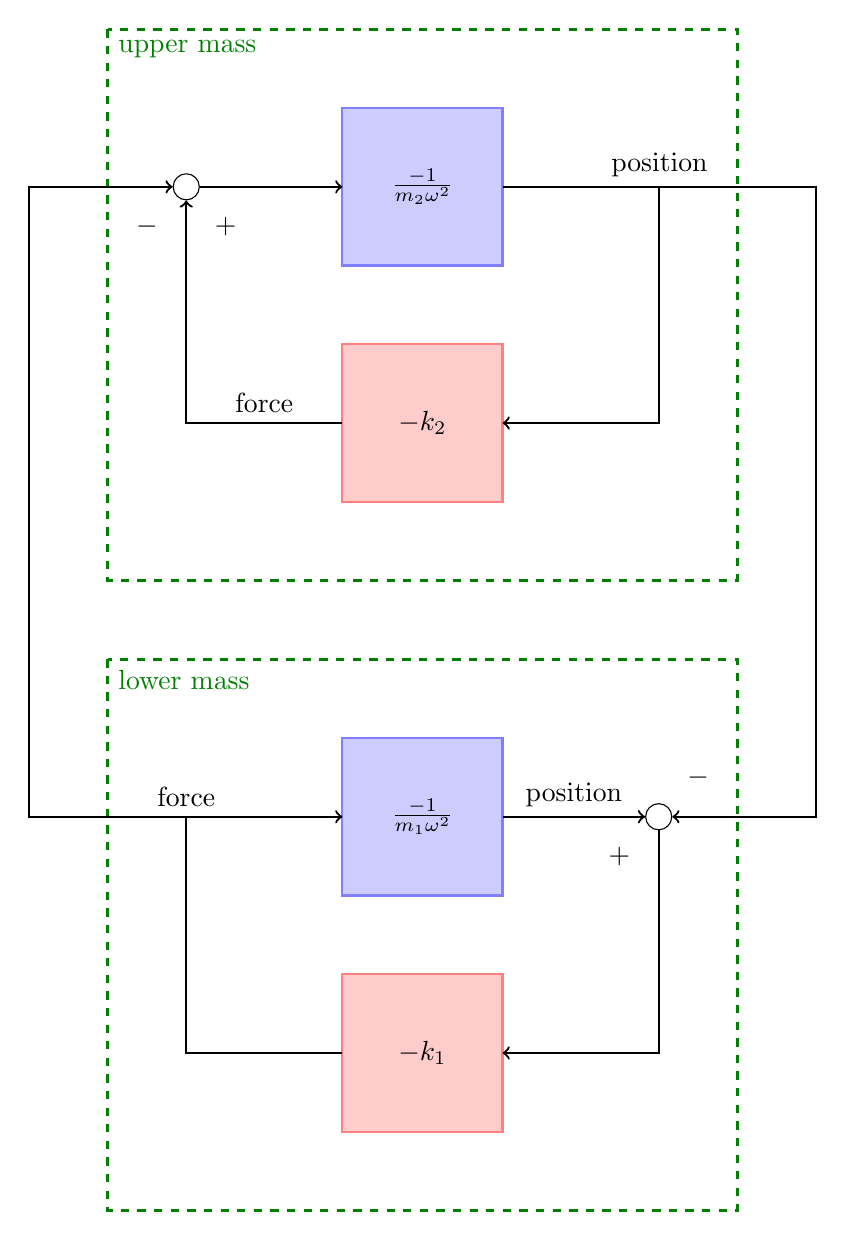
\begin{tikzpicture}
  [mass/.style={rectangle,draw=blue!50,fill=blue!20,thick,align=center,
                  outer sep=0,minimum size=2cm,text width=1.8cm},
   digital/.style={rectangle,draw=black!50,fill=black!20,thick,align=center,
                   outer sep=0,minimum size=2cm,text width=1.8cm},
   physical/.style={rectangle,draw=green!50,fill=green!20,thick,align=center,
                    outer sep=0,minimum size=2cm,text width=1.8cm},
   spring/.style={rectangle,draw=red!50,fill=red!20,thick,align=center,
                   outer sep=0,minimum size=2cm,text width=1.8cm}]
%  \renewcommand{\baselinestretch}{0.9}
%  \begin{small}
  \draw[very thick,dashed,green!50!black] (-4,2) node[anchor=north west]{upper mass} rectangle (4,-5);
  \draw[very thick,dashed,green!50!black] (-4,-6) node[anchor=north west]{lower mass} rectangle (4,-13);
  \node[spring] (spring2) at (0,-3) {$-k_2$};
  \node[mass] (mass2) at (0,0) {$\frac{-1}{m_2\omega^2}$};
  \node[spring] (spring1) at (0,-11) {$-k_1$};
  \node[mass] (mass1) at (0,-8) {$\frac{-1}{m_1\omega^2}$};
  \node[circle,draw=black] (sum2) at (-3,0) {};
  \node (plus2) at (-2.5,-0.5) {$+$};
  \node (minus2) at (-3.5,-0.5) {$-$};
  \node[circle,draw=black] (sum1) at (3,-8) {};
  \node (plus1) at (2.5,-8.5) {$+$};
  \node (minus1)  at (3.5,-7.5) {$-$};
  \node[above](labelf) at (-3,-8) {force};
  \draw[thick,->] (spring2) -- node [above] {force} (-3,-3) -- (sum2);
  \draw[thick,->] (sum2) -- (mass2);
  \draw[thick,->] (mass2) -- (3,0) |- (spring2);
  \draw[thick,->] (mass2) -- node [above] {position} (5,0) |- (sum1);
  \draw[thick,->] (sum1) |- (spring1);
  \draw[thick,->] (-3,-8) -- (-5,-8) |- (sum2);
  \draw[thick,->] (spring1) -- (-3,-11) |- (mass1);
  \draw[thick,->] (mass1) -- node [above] {position} (sum1);
%\end{small}
\end{tikzpicture}
\caption[Double Pendulum Feedback Representation]{feedback representation of
         double pendulum.
         This diagram represents the
         double pendulum feedback loops from which one can calculate the
         response of the system.
         The upper and lower masses form a feedback loop with the upper mass
         position and the lower spring (pendulum) force.
         }
\label{fig:doublesus}
\end{figure}

\begin{figure}
\centering
\tikzsetnextfilename{smallmass}
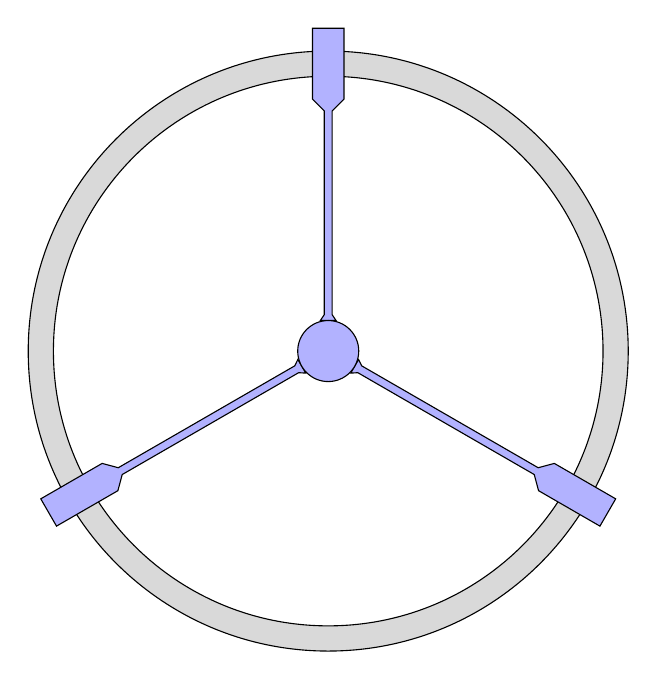
\begin{tikzpicture}
  \begin{scope}[even odd rule]
    \fill[fill=gray!30!white] (0,0) circle(3.49cm) (0,0) circle(3.81cm);
  \end{scope}
  \draw (0,0) circle(3.49);
  \draw (0,0) circle(3.81);
  \filldraw[fill=blue!30!white]
    (0.2,3.2) -- (0.2,4.1) -- (-0.2,4.1) -- (-0.2,3.2) --
    (-0.05,3.05) -- (-0.05,0.4625) -- (-0.1,0.3875) --
    (0.1,0.3875) -- (0.05,0.4625) --
    (0.05,3.05) -- cycle;
  \filldraw[fill=blue!30!white,rotate=120]
    (0.2,3.2) -- (0.2,4.1) -- (-0.2,4.1) -- (-0.2,3.2) --
    (-0.05,3.05) -- (-0.05,0.4625) -- (-0.1,0.3875) --
    (0.1,0.3875) -- (0.05,0.4625) --
    (0.05,3.05) -- cycle;
  \filldraw[fill=blue!30!white,rotate=240]
    (0.2,3.2) -- (0.2,4.1) -- (-0.2,4.1) -- (-0.2,3.2) --
    (-0.05,3.05) -- (-0.05,0.4625) -- (-0.1,0.3875) --
    (0.1,0.3875) -- (0.05,0.4625) --
    (0.05,3.05) -- cycle;
  \filldraw[fill=blue!30!white] (0,0) circle(0.3875);
\end{tikzpicture}
\caption[Small Mirror Suspension]{The small mirror suspension intermediate
         mass (gray) is a 3 inch diameter steel ring about 1/4" thick and 1"
         deep. The small mirror itself is a 7.75mm diameter fused silica
         substrate with a 5cm radius of curvature. The suspension fibers are
         monolithic to a small conical nub which is glued to the outside edge
         of the mirror.}
\label{fig:smallsus}
\end{figure}

\section{Experimental Layout}

As a reminder, we need two beams at different frequencies to couple into the
cavity.
We employ an optics path with active control on the frequency offset between
the two beams which we call the "subcarrier servo".

There are four parameters of the optical fields entering the cavity:
amplitude and frequency of each beam.
The control scheme for these parameters can be seen in figure
\ref{fig:trapcontrol1}.


\begin{figure}
\centering
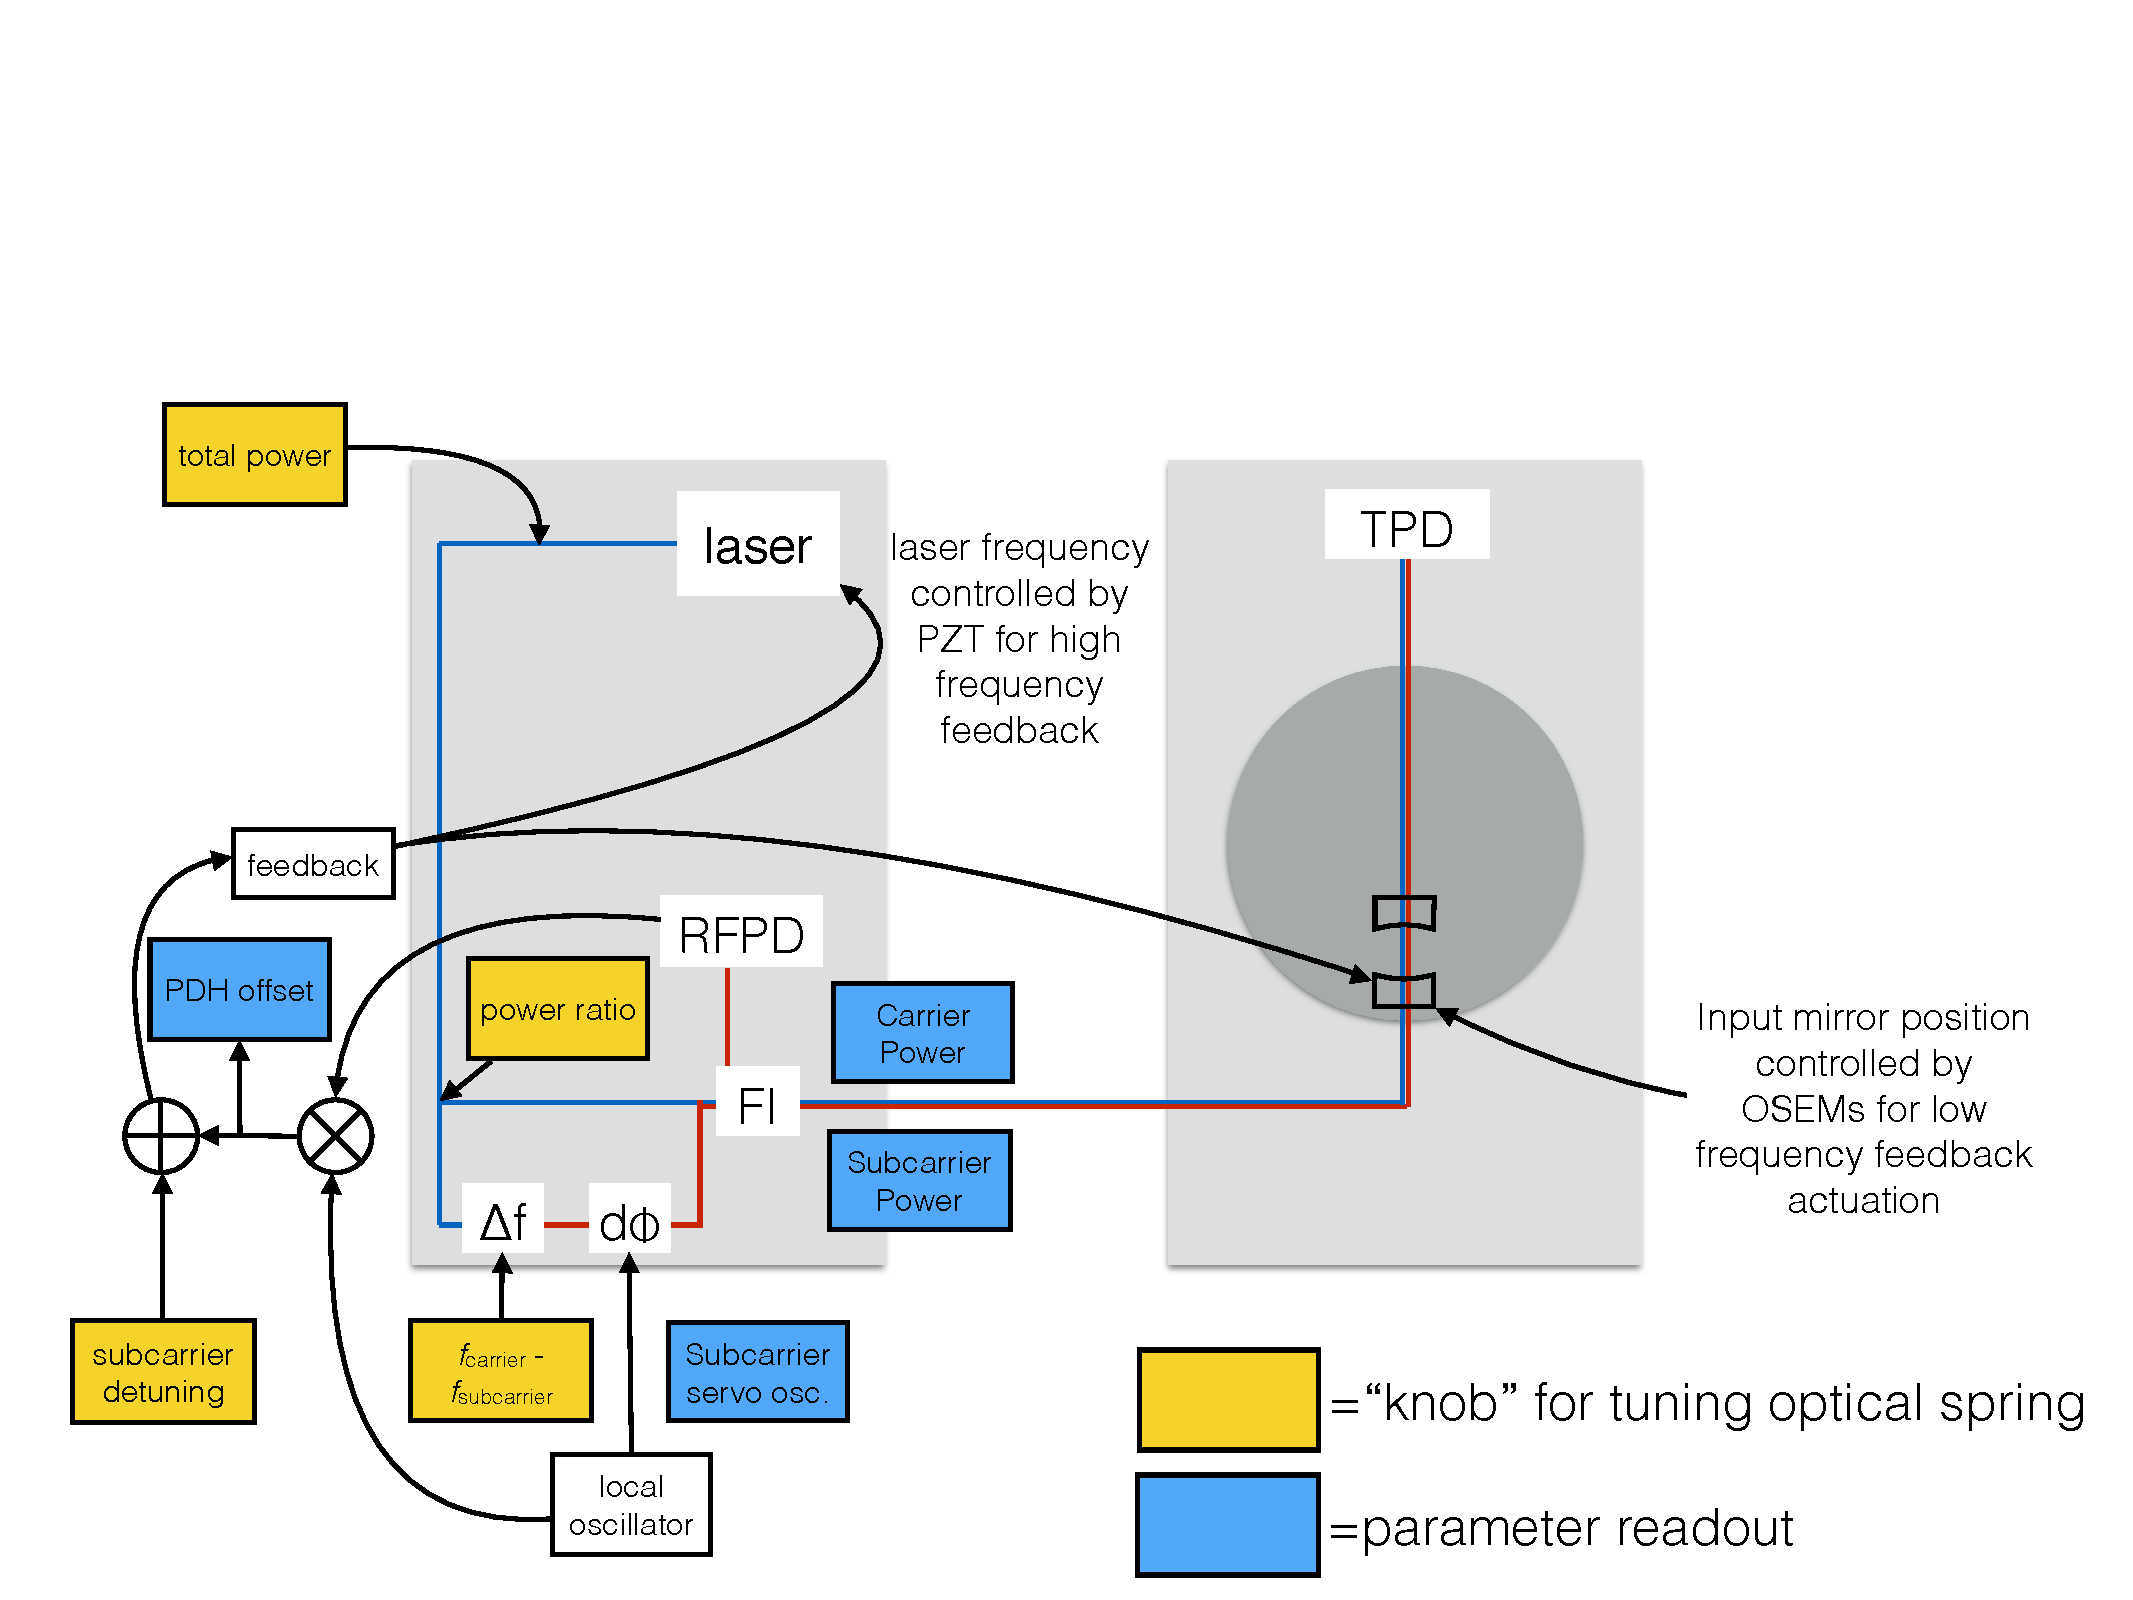
\includegraphics[width=15cm]{./figures/trapcontrol1.pdf}
\caption[Linear Trap Control]{
    trap control scheme. The figure depicts how we control the amplitude and
    frequency detuning of the two beams.
    }
\label{fig:trapcontrol1}
\end{figure}


Using the beam from our laser (ch.\ref{ch:psl}) we split into two orthogonal
polarizations. One beam we need to be at a higher power with positive detuning
(statically stable and dynamically unstable) we call the carrier beam. The
beam with less power and negative detuning we call the subcarrier.

The subcarrier optical path (fig.\ref{fig:scservo}) consists of a pair of \ac{aom}s that we use to
detune the subcarrier relative to the carrier beam.
There is also a resonant
\ac{eom} which is used to impart sidebands on the subcarrier beam for \ac{pdh}
locking.
The carrier and subcarrier are then combined using a \ac{pbs} to preserve their
orthogonal polarizations. There is a beamsplitter in the subcarrier path to pick
off the reflected light from the cavity which is used to generate the \ac{pdh}
signal. There are additional $\lambda/2$ and $\lambda/4$ waveplates at various
points in the path for polarization optimization.

%\subsection{Subcarrier Servo}
Because of our short cavity length we have a large \ac{fsr} in frequency of
about 2.14GHz.
This produces a technical problem in attempting to set the
subcarrier on the next resonance, one \ac{fsr} away.
\ac{aom}s are limited in the range of frequencies they can operate in.
The minimum is higher than the linewidth for our cavity.
The maximum is less than \ac{fsr}.

The solution for us was to set the subcarrier on the same resonance fringe
using two \ac{aom}s, each one shifting the frequency by about 80MHz in
opposite directions.
One is driven by a crystal oscillator.
The other is driven by a tunable oscillator, a \ac{vco}, which gives us the
knob to detune the subcarrier.

We produce a beat signal between the two oscillators and we lock the beat
signal to a function generator operating in the range of frequencies we are
need to detune the subcarrier with. So, now we can set directly, the carrier
to subcarrier offset frequency using the knob on the function generator.
This setup essentially eliminates frequency noise due to the crystal
oscillator, which is quite low to begin with, since we are subtracting the
same, coherent, frequency noise with the second \ac{aom}.
And the frequency noise due to the function generator is lower due to the
fact that we are using a lower frequency tunable oscillator.
Tunable oscillators generally have a frequency noise that is relative to the
set frequency.
The subcarrier servo is discussed in more detail in section
\ref{sec:scservo}.


\section{Locking Challenges}

\subsection{Optical Lever}
We found the small mirror resonances to be strong enough to prevent locking the
trapping cavity. Our solution to this was to employ an optical lever, where a
laser is reflected off the back of the small mirror and onto a \ac{qpd}.
The photodiode outputs a signal corresponding to the pitch and yaw
of the small mirror.

Using the signal from the \ac{qpd} as the error signal we feed back to the
OSEM actuators using digital filtering.
We employed resonant gain filters in the optical lever loops to damp resonance
modes as necessary to acheive stable locking.

%If you aren't careful with the position of lenses, there
%will be a coupling of the small mirror position to the photodiode signals.
%We took advantage of our carelessness and used the coupled position signal
%to feedback through resonant gain filters in the digital system and applied to
%the OSEM drives of the SOS.

\subsection{Actuation Range and Bandwidth}
\label{sec:actrangebw}
Due to seismic noise we needed a fairly wide actuation range at low frequencies.
The maximum range of the laser PZT is plus or minus 160MHz.
This corresponds to about 42nm.
As can be seen in figure \ref{fig:seismicnoise130930} there is more rms motion than this
at low frequencies.

We needed another actuation path to cover the full range of rms motion at low
frequencies.
For this we use the magnetic force from the OSEM coils.
From the OSEM coils, we calibrated a force per voltage (voltage input to current
driver board) value of $2\times 10^{-5} \mathrm{N/V}$ per coil.
With four coils we get a force range of about $\pm 8\times 10^{-4} \mathrm{N}$
for the suspension.
Most of the rms motion will come from the 18Hz resonance of the payload suspension
which is undamped.
At this frequency we are well above the pendulum frequency of the input mirror
suspension so we can treat the input mirror as a free mass.
The actuation range at this frequency is then $2\times 10^{-7}\mathrm{m}$.

While attempting to acquire lock, the cavity mirror motion is much larger than
the linewidth of the cavity.
As a result, the \ac{pdh} error signal (fig. \ref{fig:pdh}) sweeps through
rapidly.
Looking at the signal in the time domain (as with an oscilloscope), the
width of the \ac{pdh} error signal is about $50\mathrm{\mu s}$.
One can imagine that we would want a bandwidth of at least
$\approx 1/50\mathrm{\mu s} = 20\mathrm{kHz}$.
In fact a unity gain frequency of about $20\mathrm{kHz}$ turned out to work
well for acquiring lock.

To get this bandwidth a modification to the laser PZT actuation path was
required.
The high voltage amplifier for the laser PZT was limiting our bandwidth due
to it having a complex double pole at 50kHz.
This gave a rather strong rolloff in phase starting around 10kHz.
By passively adding the HV output to the HV input we could extend the
bandwidth of the PZT path.
The passive path which doesn't have the phase rolloff dominates at
high frequencies, extending the unity gain frequency we can get with
this loop.

\section{Sub-Carrier Servo}
\label{sec:scservo}
As mentioned above, we needed a way of shifting the frequency of the subcarrier
beam in relation to the carrier by $\mathcal{O}\, 100\,\mathrm{kHz}$.
We do this using \ac{aom}s by first shifting in one direction by
$80\,\mathrm{MHz}$, then shifting the opposite direction by
$80\,\mathrm{MHz} + \mathrm{offset}$.
The $80\,\mathrm{MHz}$ frequency source is a crystal oscillator.
The variable frequency source is a \ac{vco} which uses the output of a feedback
servo to modulate the frequency.
The sensor for this feedback is the demodulated beat signal of the output of
the two \ac{aom} frequency sources.
The demodulation is done by mixing the beat signal with the output of a
function generator which is set to the desired offset frequency.
See figure \ref{fig:scsfeedback} for the layout of the electronics.

\begin{figure}
\centering
\tikzsetnextfilename{scsfeedback}
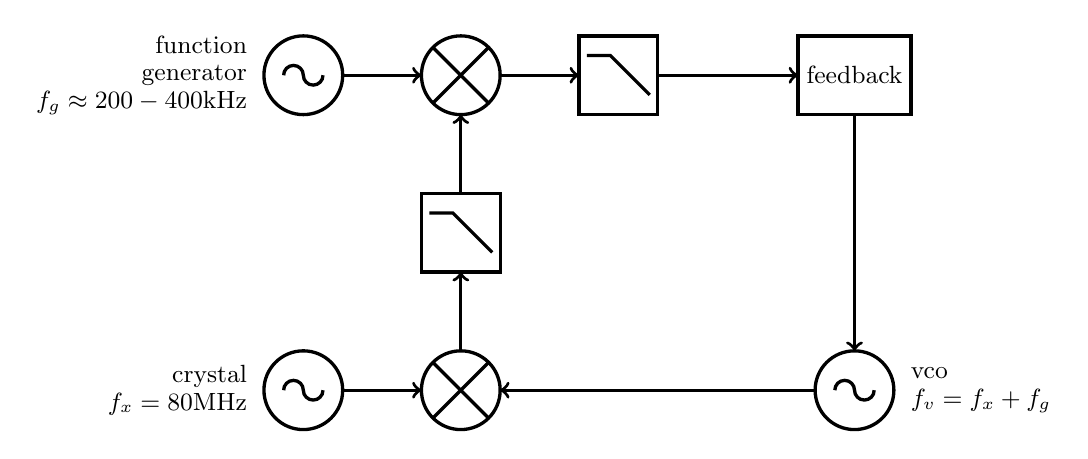
\begin{tikzpicture}
  [block/.style={rectangle,draw=black,very thick,align=center,
                  outer sep=0,minimum size=1cm,align=left},
   oscillator/.style={circle,draw=black,very thick,align=center,
                  outer sep=0,minimum size=1cm},
   digital/.style={rectangle,draw=black!50,fill=black!20,thick,align=center,
                   outer sep=0,minimum size=1cm,text width=0.9cm},
   physical/.style={rectangle,draw=green!50,fill=green!20,thick,align=center,
                    outer sep=0,minimum size=1cm,text width=0.9cm},
   spring/.style={rectangle,draw=red!50,fill=red!20,thick,align=center,
                   outer sep=0,minimum size=1cm,text width=0.9cm}]
  \renewcommand{\baselinestretch}{0.9}
  \begin{small}
  \node[block] (servo) at (2,2) {feedback};
  \node[oscillator] (mixer2) at (-3,2) {};
  \node[block] (filt1) at (-3,0) {};
  \node[block] (filt2) at (-1,2) {};
  \node[oscillator] (mixer1) at (-3,-2) {};
  \node[oscillator] (osc1) at (2,-2) {};
  \node[oscillator] (osc2) at (-5,-2) {};
  \node[oscillator] (osc3) at (-5,2) {};
  \node[align=left,anchor=west] (vco) at (2.6,-2)
    {vco\\$f_v=f_x+f_g$};
  \node[align=right,anchor=east] (crystal) at (-5.6,-2)
    {crystal\\$f_x=80 \mathrm{MHz}$};
  \node[align=right,anchor=east] (fungen) at (-5.6,2)
    {function\\generator\\$f_{g}\approx 200-400 \mathrm{kHz}$};
  \draw[very thick,->] (servo) to (osc1);
  \draw[very thick,->] (osc2) to (mixer1);
  \draw[very thick,->] (osc3) to (mixer2);
  \draw[very thick,->] (mixer1) to (filt1);
  \draw[very thick,->] (filt1) to (mixer2);
  \draw[very thick,->] (osc1) to (mixer1);
  \draw[very thick,->] (mixer2) to (filt2);
  \draw[very thick,->] (filt2) to (servo);
  \draw[very thick] (1.75,-2) arc (180:0:0.125) arc (180:360:0.125);
  \draw[very thick] (-5.25,-2) arc (180:0:0.125) arc (180:360:0.125);
  \draw[very thick] (-5.25,2) arc (180:0:0.125) arc (180:360:0.125);
  \draw[very thick] (-3,2) -- ++(45:0.5);
  \draw[very thick] (-3,2) -- ++(135:0.5);
  \draw[very thick] (-3,2) -- ++(225:0.5);
  \draw[very thick] (-3,2) -- ++(315:0.5);
  \draw[very thick] (-3,-2) -- ++(45:0.5);
  \draw[very thick] (-3,-2) -- ++(135:0.5);
  \draw[very thick] (-3,-2) -- ++(225:0.5);
  \draw[very thick] (-3,-2) -- ++(315:0.5);
  \draw[very thick] (-3.4,0.25) -- (-3.1,0.25) -- (-2.6,-0.25);
  \draw[very thick] (-1.4,2.25) -- (-1.1,2.25) -- (-0.6,1.75);
\end{small}
\end{tikzpicture}
\caption[Subcarrier Servo Electronics]{This diagram represents the
    electronic path of the subcarrier servo. This circuit locks the frequency
    of the vco to the frequency of the crystal oscillator plus an offset
    which is set by the function generator. This works by mixing the vco
    output and the crystal oscillator output together in a mixer ($\times$ in
    the diagram).
    We take the output of the first mixer and filter it with a low pass
    filter to remove the high frequency output of the mixer so that we
    are left with a sine wave at a frequency which is $f_v-f_x$.
    This low frequency signal is then mixed with the signal from the function
    generator.
    This mixer output is then the filtered with another low pass
    filter.
    The resulting error signal becomes the phase difference between the function
    generator signal and the vco, crystal difference signal, $f_v-f_x$.
    The feedback servo completes this modified phase locked loop.
    }
\label{fig:scsfeedback}
\end{figure}

%\section{Relative Power Tuning}
%
%\section{Differential Power Fluctuations}
%
%\section{Procedures}
%
%\subsection{Measure the optical losses up to the cavity}
%
%\subsection{Calibration of carrier and subcarrier photodiodes}
%We will calibrate the photodiodes while the cavity is not locked, knowing the incident beam power and the round trip losses.
%
%\begin{itemize}
%    \item Block carrier light in Mach-Zehnder path.
%    \item Turn the reflection monitor beam half-wave plate to minimize subcarrier light on the photodiode.
%    \item Block the reflection monitor beam to measure dark voltage at DCPD ($A$).
%    \item Unblock the reflection monitor beam and measure voltage at DCPD ($B$).
%    \item Unblock the carrier light and measure again ($C$)
%    \item Block subcarrier light and measure the carrier power using power meter after last steering mirror on table 1 ($D$).
%    \item Using the measured optical loss to the cavity ($L$) compute the mW/mV calibration:
%    \begin{itemize}
%        \item $\frac{D\cdot L}{C - B}$
%    \end{itemize}
%\end{itemize}

% \section{Trap Environment}
%
% The benefits of the suspension isolation would naturally be lost if the
% cavity were to be placed in air.
% Clearly we needed a decent vacuum system.
% Fortunately there was already a large bell jar in the lab.
%
%
%
% \section{Trap Control}


%\section{Noise Limitations}

%We have decided on experimental parameters with a focus on frequency noise reduction as
%this is the primary limitation as seen by Corbitt.

%Ultimately we want to have low enough technical noise so that we can turn off the active
%feedback.


\begin{figure}
\centering
\tikzsetnextfilename{roomlayout}
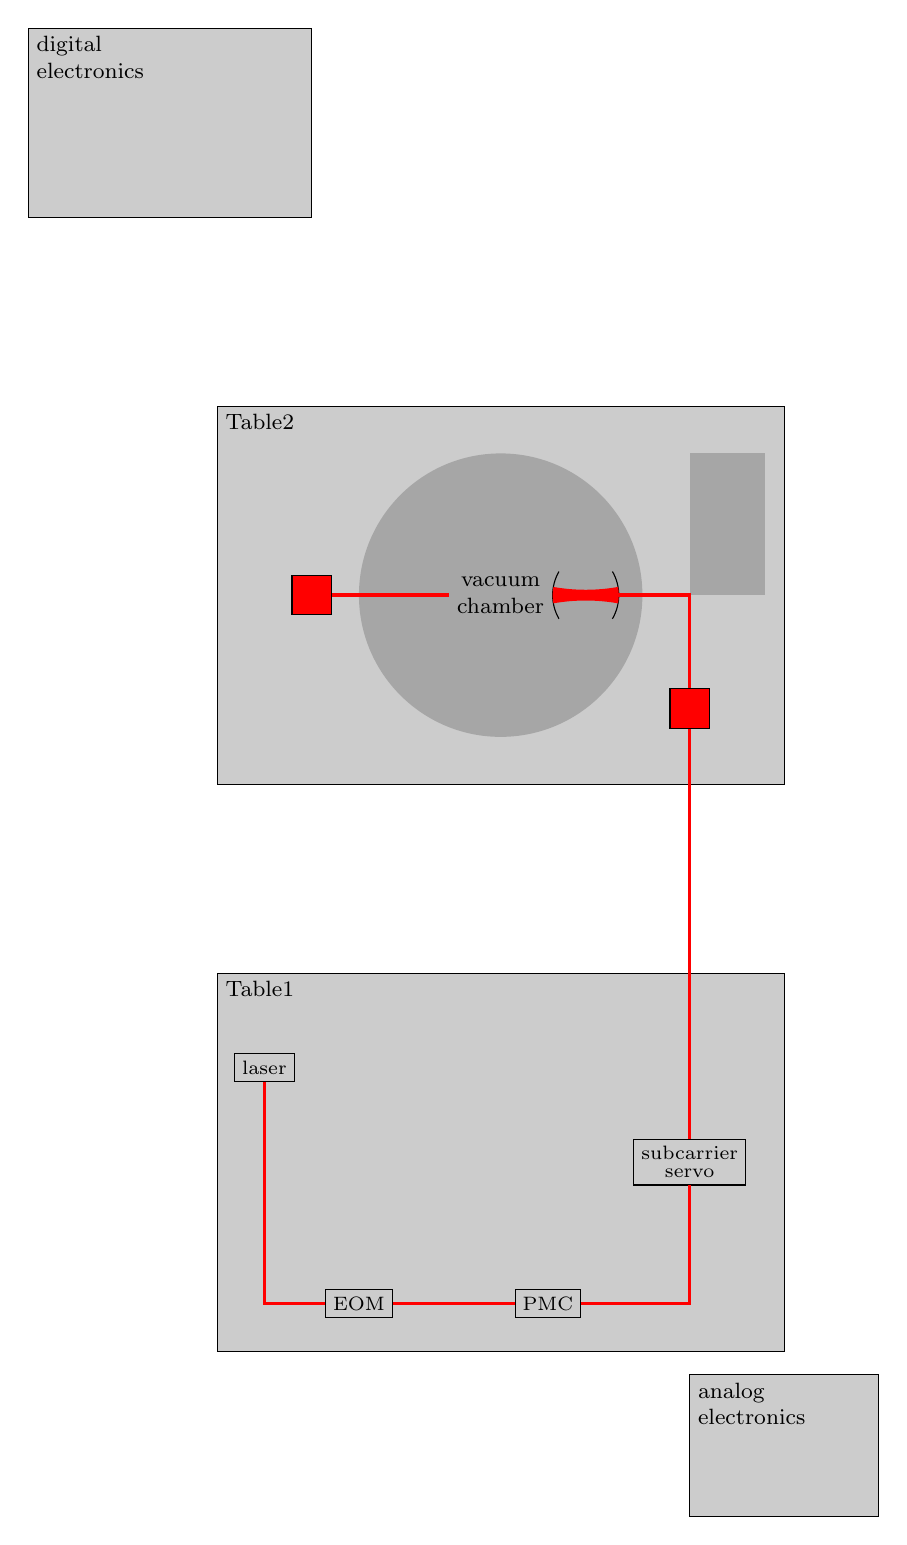
\begin{tikzpicture}[scale=1.2]
    \begin{footnotesize}
    \renewcommand{\baselinestretch}{1}
    \filldraw[fill=white!60!gray,draw=black] (8,2) rectangle (2,6)
        node[black,align=left,anchor=north west] {Table1};
    \filldraw[fill=white!60!gray,draw=black] (8,8) rectangle (2,12)
        node[black,align=left,anchor=north west] {Table2};
    \filldraw[fill=white!60!gray,draw=black] (3,14) rectangle (0,16)
        node[black,align=left,anchor=north west] { digital \\ electronics };
    \filldraw[fill=white!60!gray,draw=black] (9,0.25) rectangle (7,1.75)
        node[black,align=left,anchor=north west] { analog \\ electronics };
    \fill[white!30!gray] (5,10) circle (1.5)
        node[black,align=center] (v0) { vacuum \\ chamber };
    \fill[white!30!gray] (7,10) rectangle (7.8,11.5);
    \end{footnotesize}
    \begin{scriptsize}
    \renewcommand{\baselinestretch}{0.8}
    \draw (2.5,5) node(laser) [draw] {laser}
        (3.5,2.5) node(eom) [draw] {EOM}
        (5.5,2.5) node(pmc) [draw] {PMC}
        (7,4) node[align=center](scs) [draw] {subcarrier \\ servo}
        (7,8.8) node[align=center,fill=red,minimum height=0.5cm,minimum width=0.5cm](peris) [draw] {}
        (3,10) node[align=center,fill=red,minimum height=0.5cm,minimum width=0.5cm](peris2) [draw] {}
        (7,10) node(io) {};
    \end{scriptsize}
    \draw (5.75,10) ++(-30:0.5cm) arc (-30:30:0.5);
    \draw (5.55,10) arc (180:150:0.5)
        arc (150:210:0.5);
    \fill[red] (5.75,10) ++(-10:0.5cm) arc (-10:10:0.5)
        arc (280:260:1.971825337) arc (170:190:0.5) arc (100:80:1.971825337);
    \draw[red,very thick] (laser.south) |- (eom.west);
    \draw[red,very thick] (eom.east) |- (pmc.west);
    \draw[red,very thick] (pmc.east) -| (scs.south);
    \draw[red,very thick] (scs.north) |- (peris.south);
    \draw[red,very thick] (peris.north) |- (v0.east);
    \draw[red,very thick] (v0.west) -| (peris2.east);
\end{tikzpicture}
\caption[Room Layout]{This depicts the basic layout of how the experiment
    is situated in the lab. The red boxes on table 2 are periscopes necessary
    for getting the laser to the height of the trap cavity, and on the ouput
    side for getting back to the table height for the output optics.}
\label{fig:roomlayout}
\end{figure}

